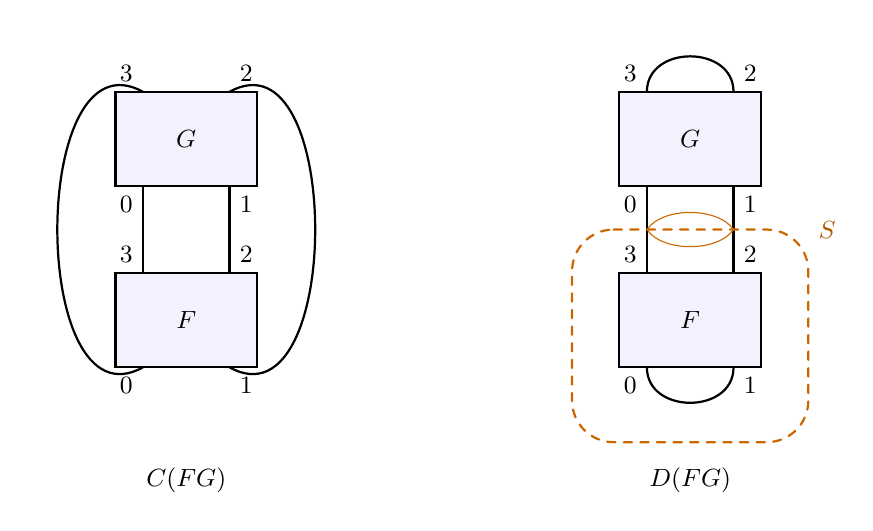
\begin{tikzpicture}[x=1cm,y=1cm,line cap=round,thick,
 every node/.style={font=\small}]
\foreach \dx/\lab in {0/{C(FG)},6.4/{D(FG)}}{
 \begin{scope}[shift={(\dx,0)}]
 \draw[fill=blue!5] (-.9,0) rectangle (.9,1.2);
 \draw[fill=blue!5] (-.9,2.3) rectangle (.9,3.5);
 \node at (0,.6) {$F$};\node at (0,2.9) {$G$};
 \foreach \x in {-.55,.55}{\draw (\x,1.2)--(\x,2.3);}
 \node[below] at (0,-1.15) {$\lab$};
 \node[below left] at (-.55,0) {$0$};
 \node[below right] at (.55,0) {$1$};
 \node[above right] at (.55,1.2) {$2$};
 \node[above left] at (-.55,1.2) {$3$};
 \node[below left] at (-.55,2.3) {$0$};
 \node[below right] at (.55,2.3) {$1$};
 \node[above right] at (.55,3.5) {$2$};
 \node[above left] at (-.55,3.5) {$3$};
 \end{scope}
}
\draw (-.55,0).. controls (-2,-.8) and (-2,4.3)..(-.55,3.5);
\draw (.55,0).. controls (2,-.8) and (2,4.3)..(.55,3.5);
\draw (5.85,0)..controls(5.85,-.6)and(6.95,-.6)..(6.95,0);
\draw (5.85,3.5)..controls(5.85,4.1)and(6.95,4.1)..(6.95,3.5);
\draw[orange!80!black,dashed,rounded corners=15pt]
 (4.9,1.75)--(7.9,1.75)--(7.9,-.95)--(4.9,-.95)--cycle;
\node[right,orange!70!black] at (7.9,1.75) {$S$};
\draw[orange!80!black,thin] (5.85,1.75)..controls(6.05,1.46)and(6.75,1.46)..(6.95,1.75);
\draw[orange!80!black,thin] (5.85,1.75)..controls(6.05,2.04)and(6.75,2.04)..(6.95,1.75);
\end{tikzpicture}
